\documentclass{article}

\usepackage[letterpaper,portrait,top=0.4in, left=0.6in, right=0.6in, bottom=1in]{geometry}

\usepackage{amsmath, amsfonts, amsthm, amssymb}
\usepackage{graphicx, float}
\usepackage{mathtools}
\usepackage{titlesec}
\usepackage{interval}
\usepackage{titling}
\usepackage{vwcol}
\usepackage{esdiff}
\usepackage{empheq}
\usepackage{cancel}
\usepackage{pdfpages}
\usepackage{graphicx}
\usepackage[export]{adjustbox}

\intervalconfig {
	soft open fences
}

\newcommand{\alignedintertext}[1]{%
	\noalign{%
		\vskip\belowdisplayshortskip
		\vtop{\hsize=\linewidth#1\par
		\expandafter}%
		\expandafter\prevdepth\the\prevdepth
	}%
}

%opening
\title{Problem Set \#45}
\author{Jayden Li}
\date{January 24, 2024}

\begin{document}

\newgeometry{top=0in, left=0.6in, right=0.6in, bottom=0.2in}

\fontsize{12pt}{12pt}\selectfont

\maketitle

\section*{Problem 2}
\vspace{-15pt}
\centering
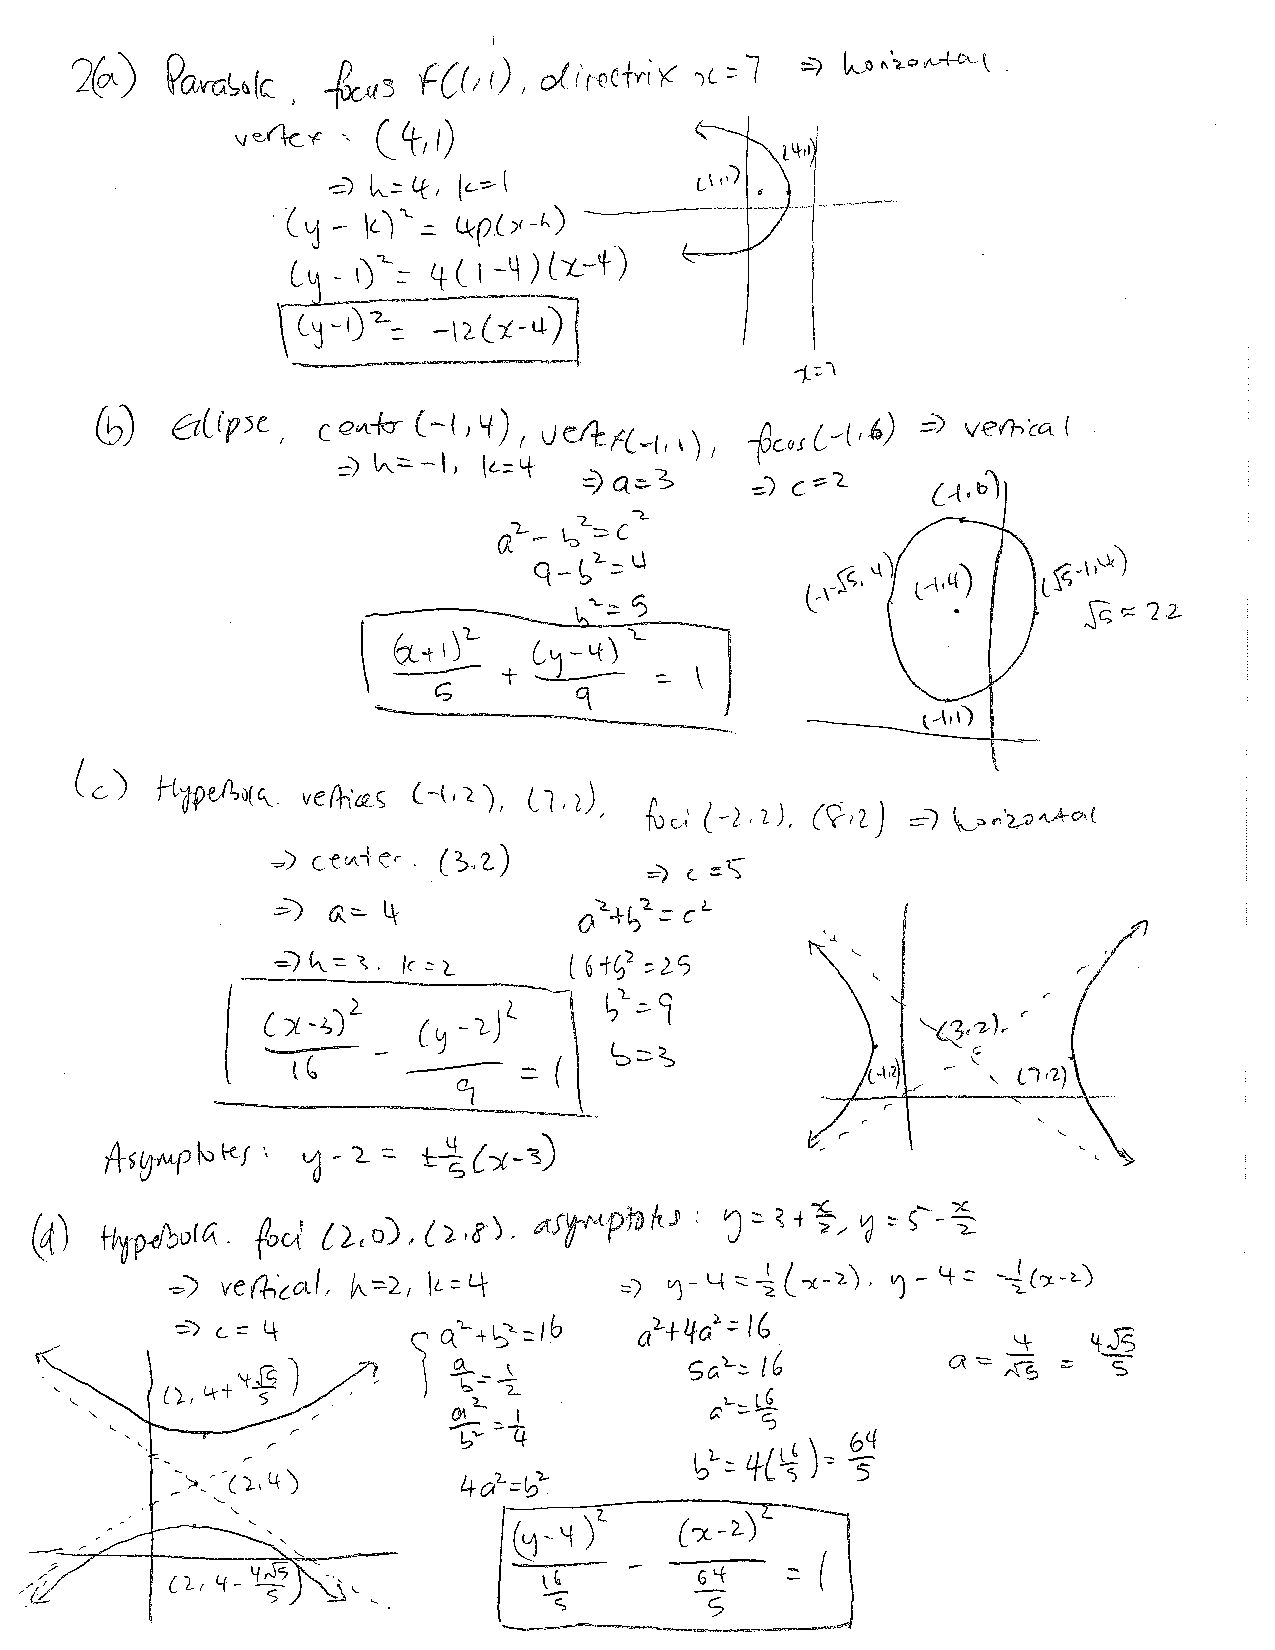
\includegraphics[scale=0.76,page=1]{scan.pdf}
\flushleft

\restoregeometry
\section*{Problem 3}
\begin{itemize}
\item[(a)]
\textbf{Ellipse}. If $k>16$, then $k>0$ and $k-16>0$.

\item[(b)]
\textbf{Hyperbola}. If $0<k<16$, then $k>0$ and $k-16<0$.

\item[(c)]
\textbf{No real values}. If $k<0$, then $k<0$ and $k-16<0$. $x^2>0$ and $y^2>0$ for $x,y\in\mathbb{R}$. Therefore, $\dfrac{x^2}{k}$ and $\dfrac{y^2}{k-16}$ are negative and the sum of two negative numbers cannot be $1$.

\item[(d)]
	\begin{itemize}
	\item[(a)]
		$\displaystyle \frac{x^2}{k}+\frac{x^2}{x-16}=1 \implies a=\sqrt{k},b=\sqrt{k-16} \implies c=\sqrt{a^2-b^2}=\sqrt{k-(k-16)}=4$. The focus of the ellipse is at $(4,0)$ and $(-4,0)$ for all $k>16$.

	\item[(b)]
		$\displaystyle \frac{x^2}{k}+\frac{x^2}{x-16}=1 \implies \frac{x^2}{k}-\frac{x^2}{16-x}=1 \implies a=\sqrt{k},b=\sqrt{16-k} \implies c=\sqrt{a^2+b^2}=\sqrt{k+(16-k)}=4$. The focus of the hyperbola is at $(4,0)$ and $(-4,0)$ for all $0<k<16$.
	\end{itemize}
\end{itemize}

\section*{Problem 6}
\begin{itemize}
\item[(a)]
	\begin{minipage}[t]{\linewidth}
		\centering
		\setlength{\abovedisplayskip}{0pt}
		\begin{minipage}[t]{0.31\linewidth}
		\begin{align*}
			y^2&=4px \\
			\diff{}{x}y^2&=\diff{}{x}4px \\
			2y\diff{y}{x}&=4p \\
			\diff{y}{x}&=\frac{2p}{y}
		\end{align*}
		\end{minipage}
		\begin{minipage}[t]{0.31\linewidth}
		\begin{align*}
			y-y_0&=\frac{2p}{y_0}(x-x_0) \\
			y_0y-y_0^2&=2p(x-x_0) \\
			y_0y&=2px-2px_0+4px_0 \\
			y_0y&=2px+2px_0 \\
			\Aboxed{y_0y&=2p(x+x_0)}
		\end{align*}
		\end{minipage}
	\end{minipage}

\item[(b)]
	\phantom{}

	\centering
	\begin{minipage}[t]{0.2\linewidth}
		\begin{align*}
			y_0y&=2p(x+x_0) \\
			y&=\frac{2px}{y_0}+\frac{4px_0}{2y_0} \\
			y&=\frac{2px}{y_0}+\frac{y_0^{\cancel{2}}}{2\cancel{y_0}} \\
			\Aboxed{y&=\frac{2px}{y_0}+\frac{y_0}{2}} \\
		\end{align*}
	\end{minipage}
	\begin{minipage}[t]{0.55\linewidth}
		\centering
    	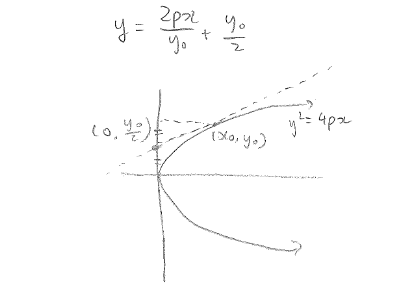
\includegraphics[valign=t,scale=0.9]{q6b.png}
	\end{minipage}
	\flushleft
	
\end{itemize}

\section*{Problem 7}
\centering
\vspace*{-10pt}
\includegraphics*[width=\linewidth]{q7.png}
\flushleft

\end{document}